\documentclass{beamer}
\usepackage{listings,bm}
\usepackage{hyperref}
\usepackage{animate}
\usepackage{tikz}
\usetikzlibrary{positioning,shadows,arrows,shapes,calc}
\usepackage{tipa}
\DeclareMathOperator*{\softmax}{softmax}
\newcommand{\ipa}[1]{\fontfamily{cmr}\selectfont\textipa{#1}}
\def\labelenumi\theenumi
\usepackage{graphicx}
\usepackage{amsmath}
\mode<presentation>{\usetheme{Frankfurt}}
\AtBeginSection
{
  \begin{frame}<beamer>
    \frametitle{Outline}
    \tableofcontents[currentsection,currentsubsection]
  \end{frame}
}
\title{Lecture 22: Unsupervised and Self-Supervised Learning}
\author{Mark Hasegawa-Johnson\\These slides are in the public domain}
\date{ECE 417: Multimedia Signal Processing}
\institute{University of Illinois}
\titlegraphic{\includegraphics[width=0.3in]{exp/block-I-primary.png}}
\begin{document}

% Title
\begin{frame}
  \maketitle
\end{frame}

% Title
\begin{frame}
  \tableofcontents
\end{frame}

%%%%%%%%%%%%%%%%%%%%%%%%%%%%%%%%%%%%%%%%%%%%
\section[Overview]{Unsupervised Learning}
\setcounter{subsection}{1}

\begin{frame}
  \frametitle{What is Unsupervised Learning?}

  \begin{itemize}
  \item {\bf Supervised learning:} given pairs of data, $(x_i,y_i)$,
    learn a mapping $f(x)\approx y$.
  \item {\bf Unsupervised learning:} given unlabeled training
    examples, $x_i$, learn something about them.
    \begin{itemize}
    \item Can $x_i$ be decomposed into signal + noise?
    \item Can we group the $x$'s into ``natural classes,'' i.e.,
      groups of tokens that are similar to one another?
    \item Can we design a classifier that puts $x_i$ into its natural
      class?
    \end{itemize}
  \end{itemize}
\end{frame}

\begin{frame}
  \frametitle{Some types of unsupervised learning}

  \begin{itemize}
  \item {\bf Manifold learning:} decompose $x_i$ into signal + noise
  \item {\bf Clustering:} group the $x$'s into natural classes
  \item {\bf Self-supervised learning:} learn a classifier that
    puts $x_i$ into its natural class
  \end{itemize}
\end{frame}

%%%%%%%%%%%%%%%%%%%%%%%%%%%%%%%%%%%%%%%%%%%%
\section[Manifolds]{Manifold Learning}
\setcounter{subsection}{1}

\begin{frame}
  \begin{columns}
    \begin{column}{0.5\textwidth}
      \begin{itemize}
      \item Signals lie on a manifold if some perturbations are
        impossible (``perpendicular'' to the manifold)
      \item If signals are on a manifold, then perturbations
        perpendicular to the manifold are always noise, and can be
        ignored.
      \end{itemize}
    \end{column}
    \begin{column}{0.5\textwidth}
      \begin{center}
        \animategraphics[loop,controls,width=\textwidth]{30}{exp/Insect_on_a_torus-}{0}{464}

        \begin{tiny}
          CC-SA 4.0, \url{https://commons.wikimedia.org/wiki/File:Insect_on_a_torus_tracing_out_a_non-trivial_geodesic.gif}
        \end{tiny}
      \end{center}
    \end{column}
  \end{columns}
\end{frame}

\begin{frame}
  \frametitle{Speech Manifolds}

  \begin{itemize}
  \item {\bf The signal manifold:} Each sample is $s[n]=d[n]+\sum a_m
    s[n-m]$.  The excitation, $d[n]$, is sparse: only about 10\% of
    its samples should be nonzero.
  \item {\bf The articulatory manifold:} The formant frequencies and
    bandwidths change slowly as a function of time, because they are
    shaped by positions of the tongue, jaw, and lips, and those things
    have mass.
  \end{itemize}
\end{frame}

\begin{frame}
  \begin{columns}
    \begin{column}{0.5\textwidth}
      {\bf The signal manifold:}
      \begin{itemize}
      \item When CNNs are learned directly from the speech samples,
        the first-layer filters tend to look like a Fourier transform.
      \item Example at right: Figure 2, ``Multichannel Signal
        Processing with Deep Neural Networks for Automatic Speech
        Recognition,'' Sainath et al., 2017, (c) IEEE
      \end{itemize}
    \end{column}
    \begin{column}{0.5\textwidth}
      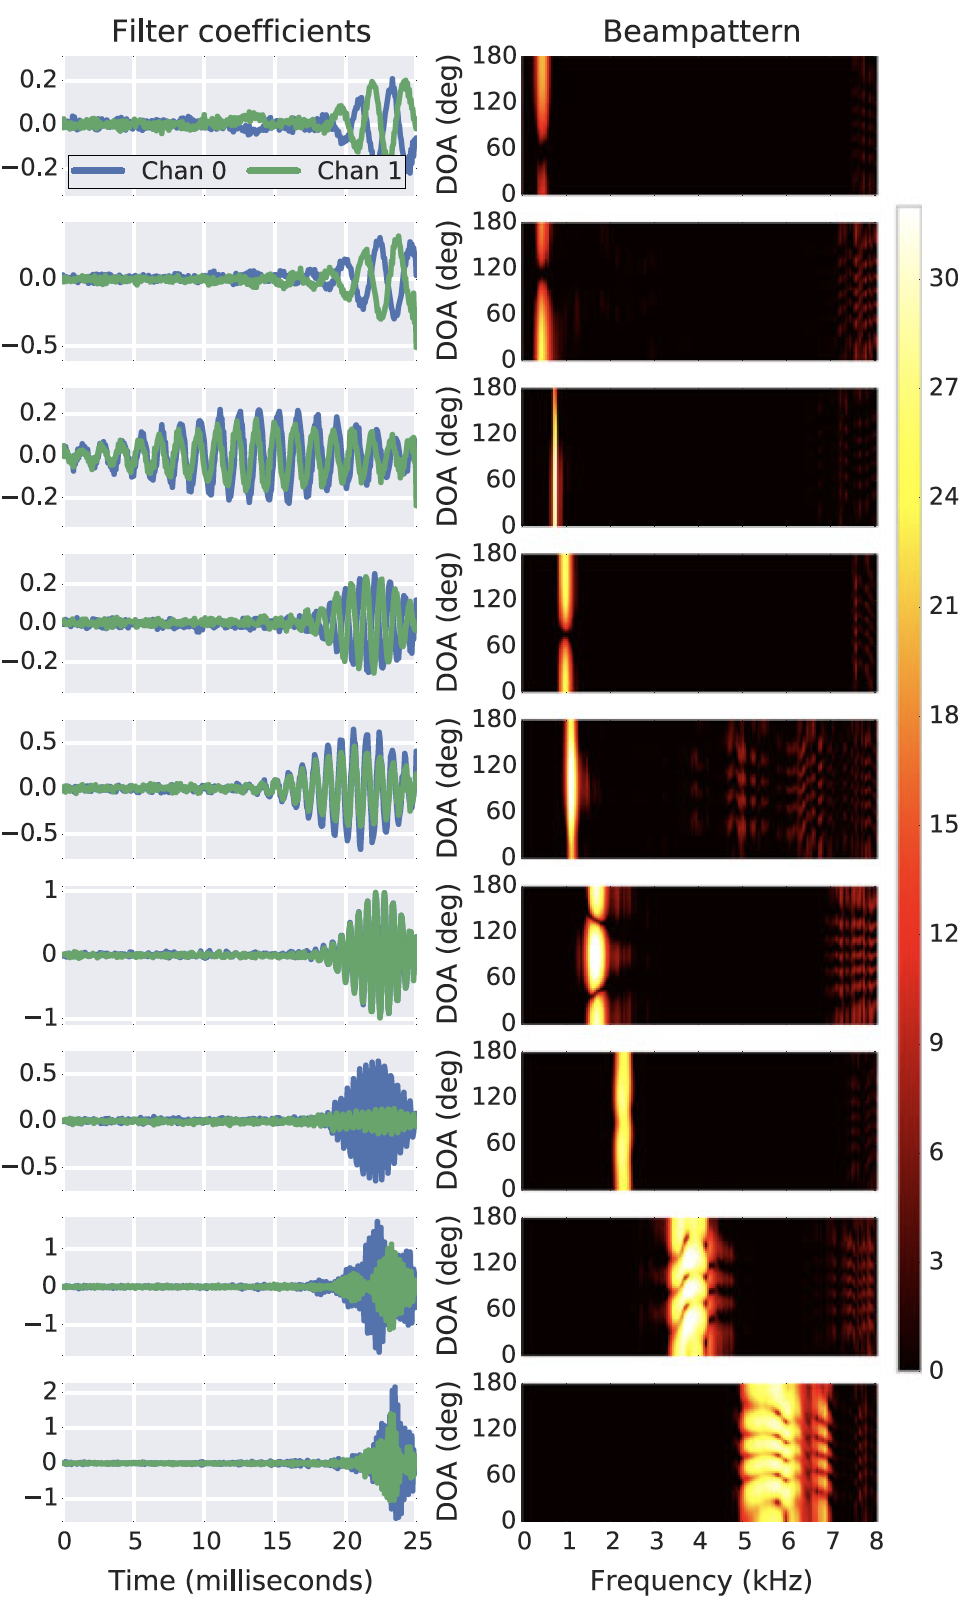
\includegraphics[height=\textheight]{figs/sainath2017fig2.png}
    \end{column}
  \end{columns}
\end{frame}

\begin{frame}
  \frametitle{The articulatory manifold (Deng et al., Interspeech 2010)}

  \centerline{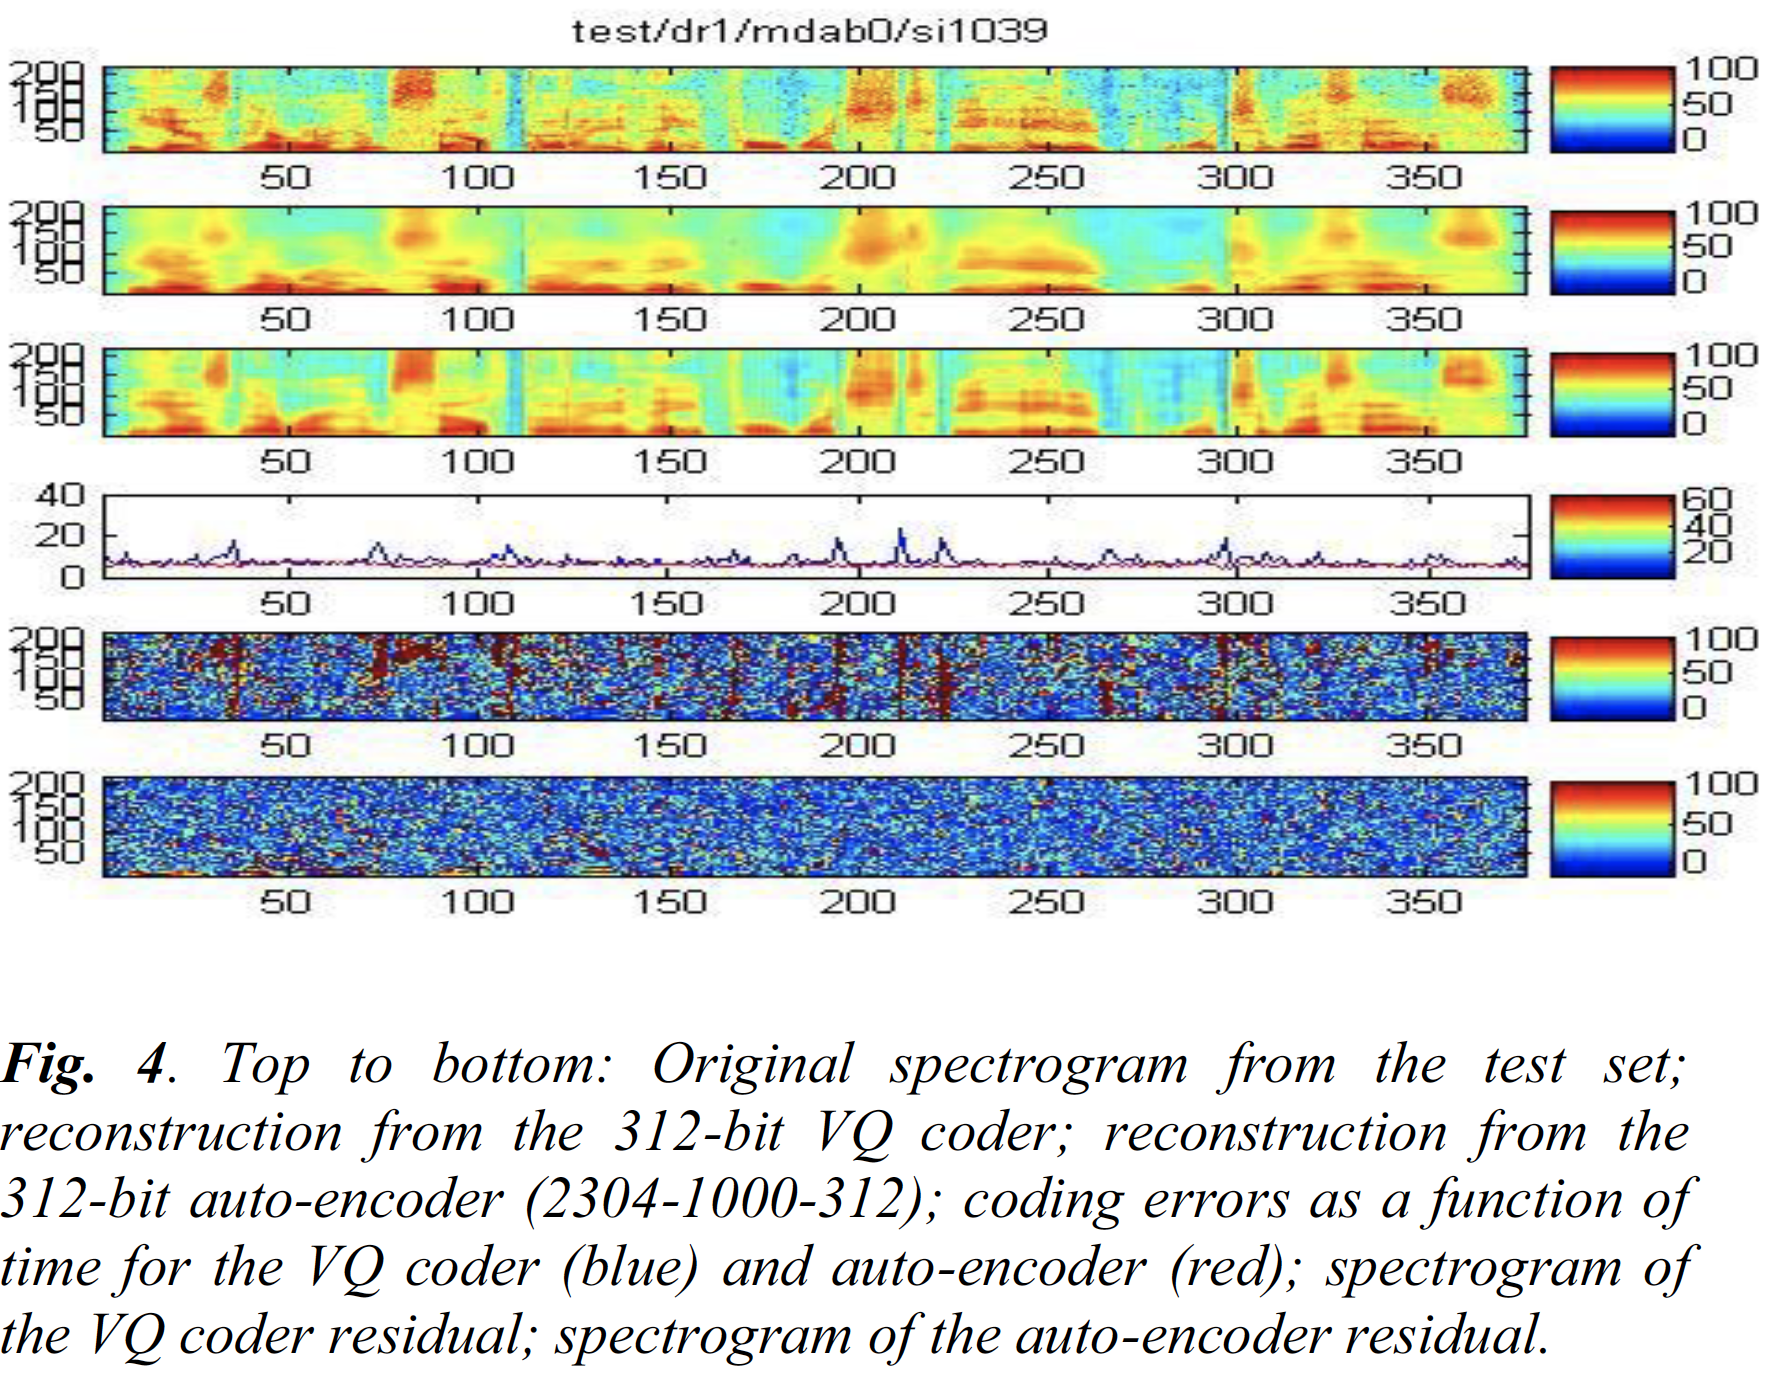
\includegraphics[height=0.88\textheight]{figs/deng2010fig4.png}}
\end{frame}

\begin{frame}
  \frametitle{PCA: Manifold = Hyperplane}
  \begin{columns}
    \begin{column}{0.5\textwidth}
      If the signal is constrained to lie on a hyperplane, then the
      hyperplane can be found using principal components analysis
      (PCA).
    \end{column}
    \begin{column}{0.5\textwidth}
      \begin{center}
        \includegraphics[width=\textwidth]{exp/PCA_seagrass.png}

        \begin{tiny}
          CC-SA 4.0, \url{Principal_Component_Analyses_for_the_morphological_and_molecular_surveys_of_seagrass_meadows}
        \end{tiny}
      \end{center}
    \end{column}
  \end{columns}
\end{frame}
  
\begin{frame}
  \frametitle{PCA is computed by a one-layer autoencoder}
  \begin{columns}
    \begin{column}{0.5\textwidth}
      A one-layer autoencoder (one matrix multiply, then a hidden
      layer, then the inverse of the same matrix) computes the PCA of
      its input.
    \end{column}
    \begin{column}{0.5\textwidth}
      \begin{center}
        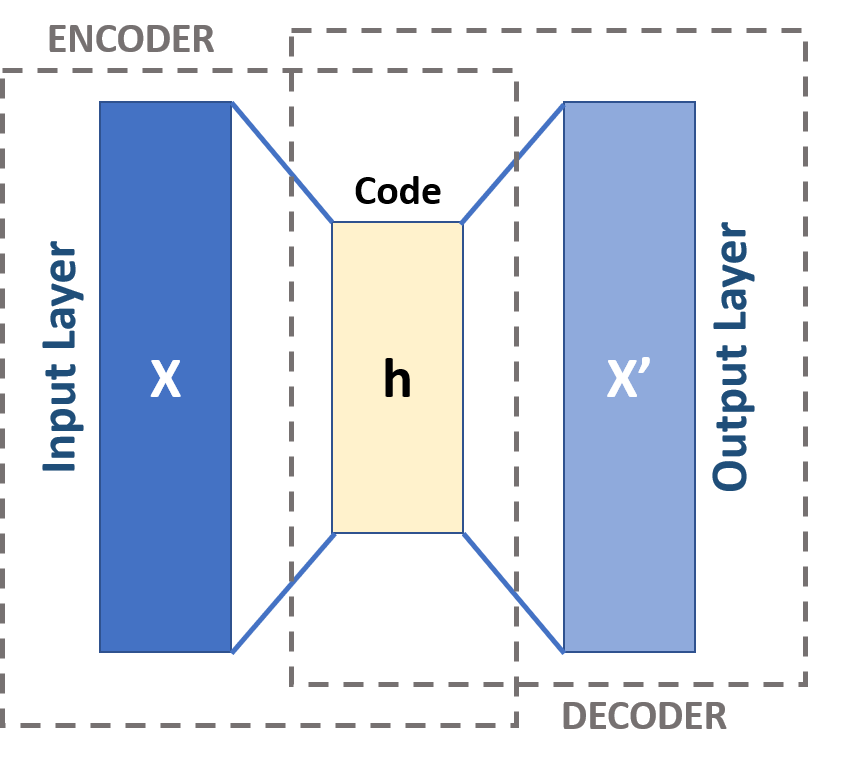
\includegraphics[width=\textwidth]{exp/Autoencoder_schema.png}

        \begin{tiny}
          CC-SA 4.0, \url{https://commons.wikimedia.org/wiki/File:Autoencoder_schema.png}
        \end{tiny}
      \end{center}
    \end{column}
  \end{columns}
\end{frame}
  
        
\begin{frame}
  \frametitle{Two-layer autoencoder can compute a nonlinear manifold}
  \begin{columns}
    \begin{column}{0.5\textwidth}
      \begin{itemize}
      \item A two-layer autoencoder constrains the data, $x$, to lie
        on a {\bf nonlinear} manifold of dimension = $\text{dim}(z)$.
      \item The first layer nonlinearly transforms the input, then the
        second layer computes PCA of the result.
      \end{itemize}
    \end{column}
    \begin{column}{0.5\textwidth}
      \begin{center}
        \includegraphics[width=\textwidth]{exp/Autoencoder_structure.png}

        \begin{tiny}
          CC-SA 4.0, \url{https://commons.wikimedia.org/wiki/File:Autoencoder_structure.png}
        \end{tiny}
      \end{center}
    \end{column}
  \end{columns}
\end{frame}

\begin{frame}
  \frametitle{Summary: Manifolds}

  \begin{itemize}
  \item Speech lies on manifolds of (at least) two timescales
    \begin{itemize}
    \item {\bf Signal manifold:} samples are predictable from previous samples
    \item {\bf Articulatory manifold:} formant frequencies and
      bandwidths are predictable from previous formants and bandwidths
    \end{itemize}
  \item By learning to represent the manifolds, the early layers of an ASR
    learn to reject irrelevant variation (noise) and keep only relevant variation (signal)
  \item Autoencoders explicitly learn manifolds
  \end{itemize}
\end{frame}
        
%%%%%%%%%%%%%%%%%%%%%%%%%%%%%%%%%%%%%%%%%%%%
\section[Clustering]{Clustering}
\setcounter{subsection}{1}

\begin{frame}
  \begin{columns}
    \begin{column}{0.3\textwidth}
      \begin{itemize}
      \item The idea of {\bf clustering} is to group the observed data
        into {\bf natural classes} (things that sound similar).
      \item After grouping them into natural classes, we can then
        assign a label to each natural class.
      \end{itemize}

      {\tiny Peterson and Barney, 1952.  Copyright
      Acoustical Society of America.}
    \end{column}
    \begin{column}{0.7\textwidth}
      \begin{center}
        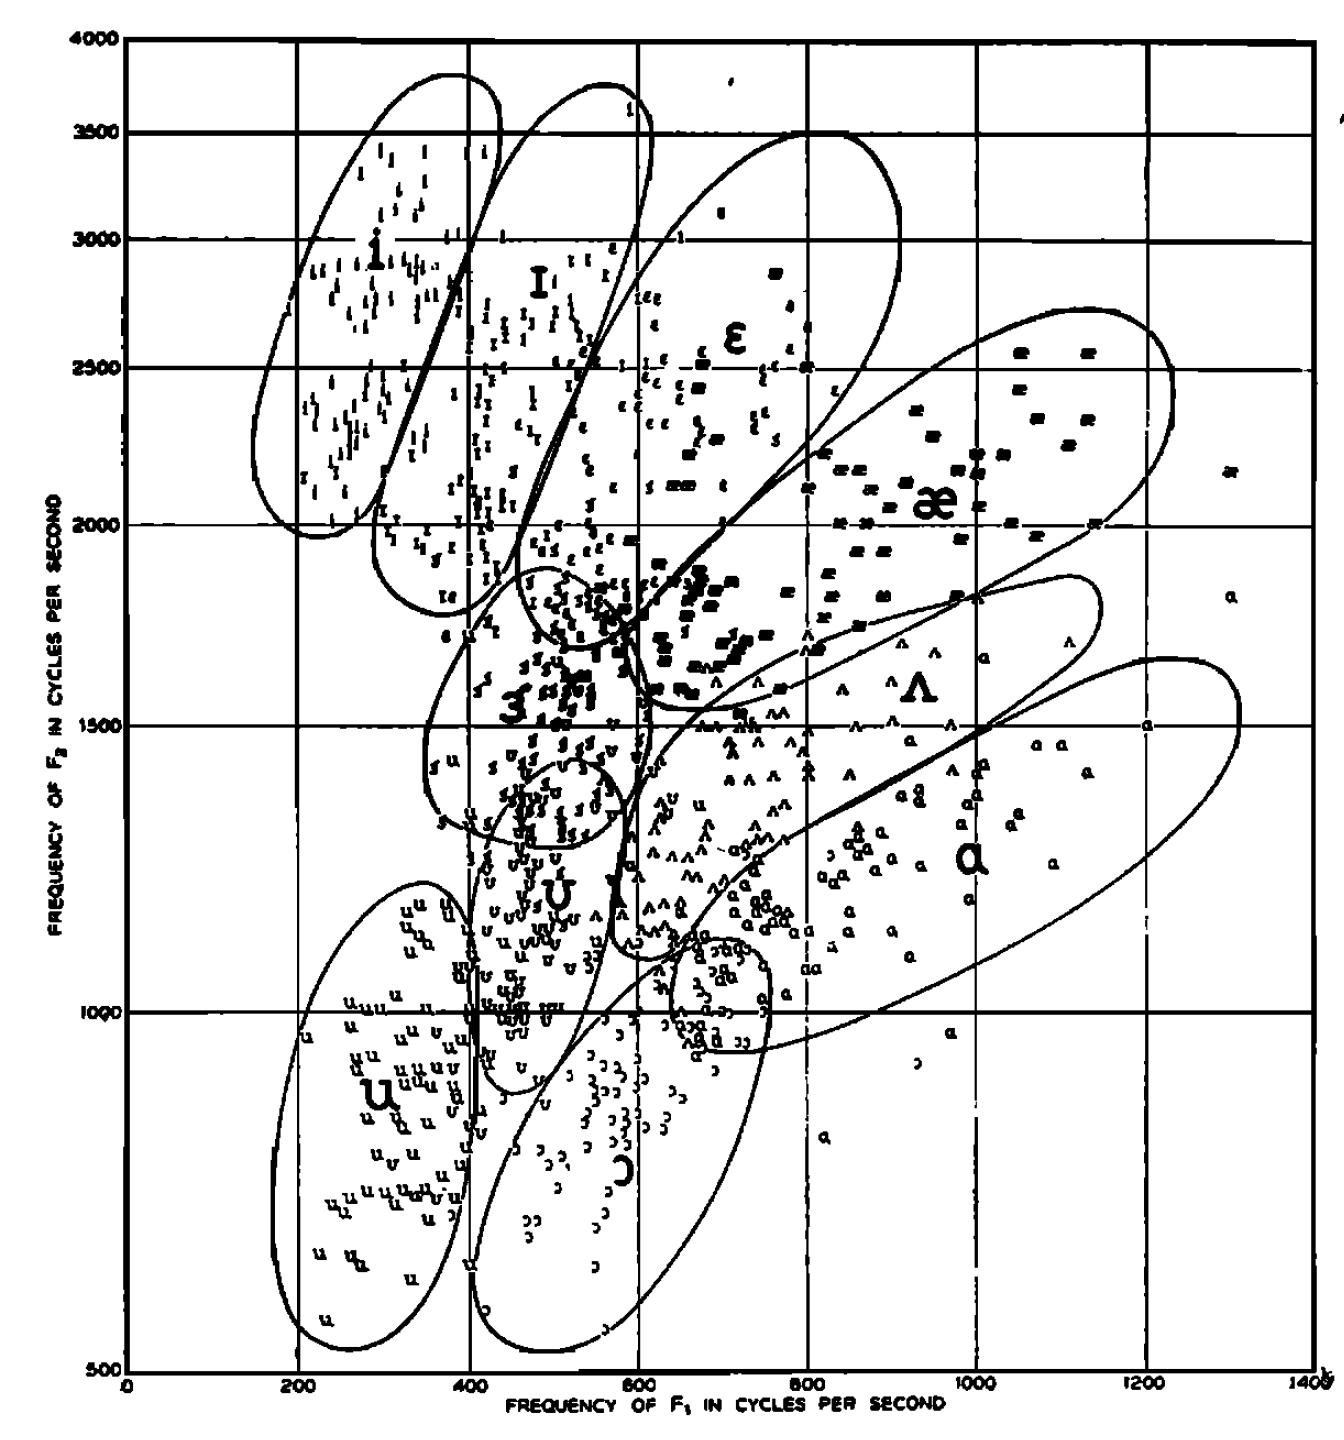
\includegraphics[width=\textwidth]{figs/peterson1952fig8.png}
      \end{center}
    \end{column}
  \end{columns}
\end{frame}

\begin{frame}
  \frametitle{K-Means Clustering {\tiny (\url{https://en.wikipedia.org/wiki/K-means_clustering})}}
  \begin{columns}
    \begin{column}{0.5\textwidth}
      {\bf Step 0:} Choose random initial ``means''
      \centerline{\includegraphics[width=0.6\textwidth]{exp/K_Means_Step_1.png}}

      {\bf Step 1:} Group each token with its closest mean
      \centerline{\includegraphics[width=0.6\textwidth]{exp/K_Means_Step_2.png}}
    \end{column}
    \begin{column}{0.5\textwidth}
      {\bf Step 2:} Mean = average of its tokens
      \centerline{\includegraphics[width=0.6\textwidth]{exp/K_Means_Step_3.png}}

      {\bf Step 3:} Repeat step 1
      \centerline{\includegraphics[width=0.6\textwidth]{exp/K_Means_Step_4.png}}
    \end{column}
  \end{columns}
\end{frame}

\begin{frame}
  \frametitle{Gaussian Mixture Modeling}

  Gaussian mixture modeling is like K-means, except that each cluster
  has a different covariance matrix.  Result can be very similar to a
  natural vowel space.

  \begin{center}
    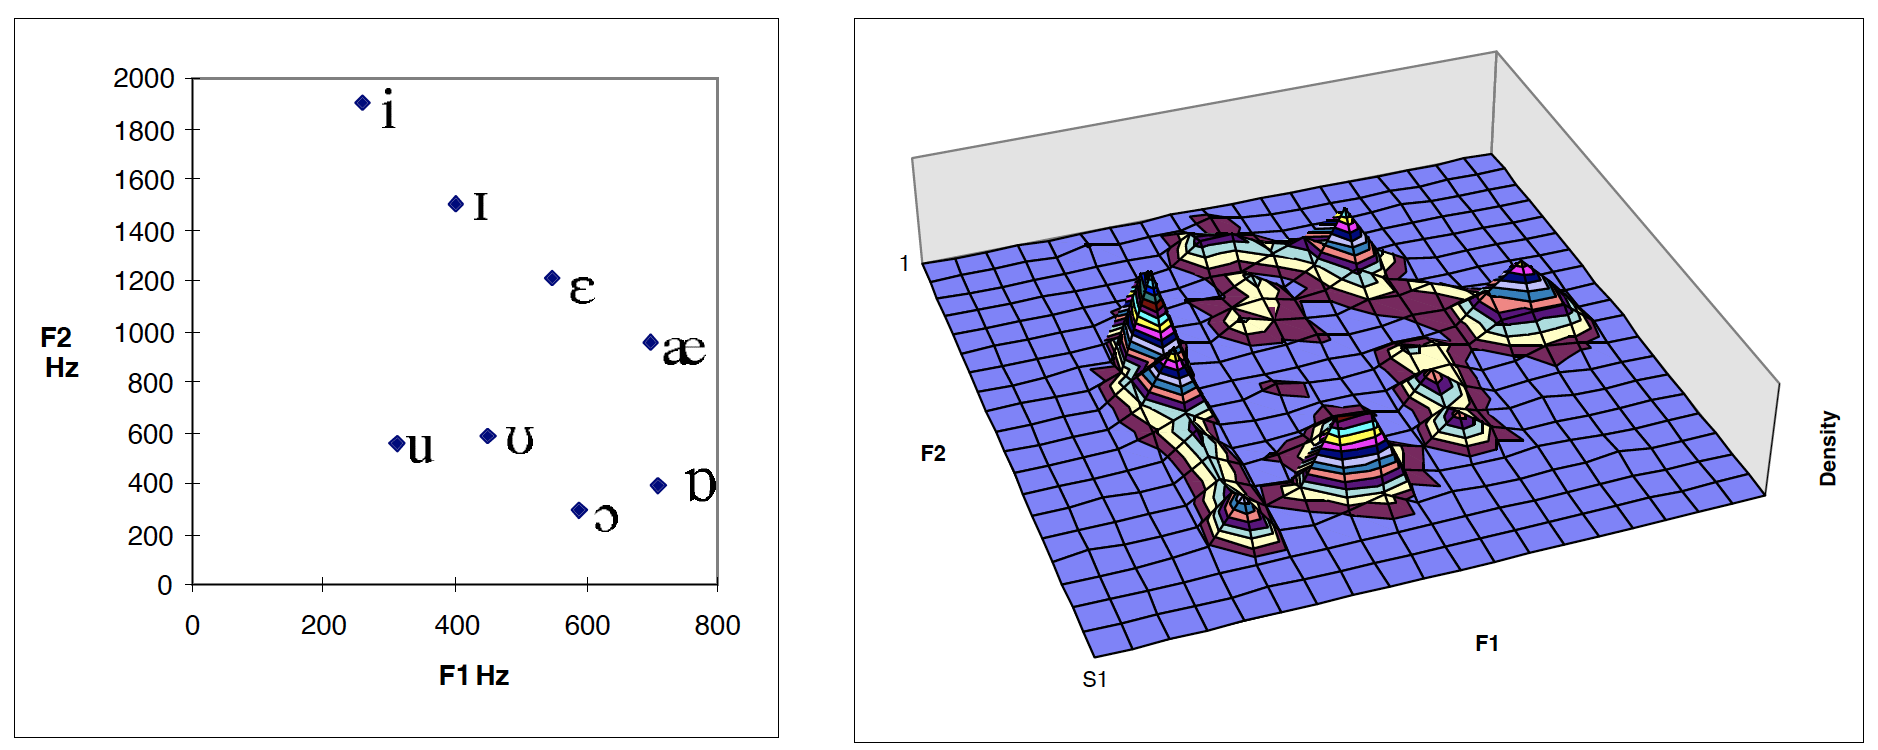
\includegraphics[width=\textwidth]{figs/aylett1998fig1.png}

    \begin{tiny}
      Fig. 1, ``Building a Statistical Model of the Vowel Space for Phoneticians,''
      (c) Matthew Aylett, 1998
    \end{tiny}
  \end{center}
\end{frame}

%%%%%%%%%%%%%%%%%%%%%%%%%%%%%%%%%%%%%%%%%%%%
\section[Self-Supervision]{Self-Supervised Classifier Learning: Matched-Filter Example}
\setcounter{subsection}{1}

\begin{frame}
  \frametitle{Unsupervised Classifier Example}

  In 1965, Scudder (``Probability of Error of Some Adaptive
  Pattern-Recognition Machines'') considered the following example:
  \begin{itemize}
  \item $Z_1,\ldots,Z_n,\ldots$ is a series of vectors.
  \item Each vector either contains signal + noise ($Z_n=X+N_n$),
    or just noise ($Z_n=N_n$).
  \item The signal, $X$, is the same every time it appears, but it is
    unknown.
  \item The noise, $N_n$, is zero-mean Gaussian noise with covariance
    matrix $K_N=\sigma^2I$.
  \end{itemize}
\end{frame}

\begin{frame}
  \frametitle{Unsupervised Classifier Example}

  Here are the questions Scudder asked:
  \begin{enumerate}
  \item Suppose a classifier was asked to determine whether or not the
    pattern is present.  What it the optimum decision rule?
  \item Suppose a classifier was trained {\bf without any training
    labels}.  Can it learn the optimum decision rule?
  \end{enumerate}
\end{frame}


\begin{frame}
  \frametitle{The Supervised Case}

  First, consider the supervised case.  We don't know $X$, but we are
  given labels: $\theta_n=1$ if  $Z_n=X+N_n$, otherwise $\theta_n=0$.
  The optimum decision rule turns out to be:
  \begin{itemize}
  \item Update the matched filter covariance estimate:
    \begin{displaymath}
      K_{n+1} = \left(K_n^{-1}+\theta_n K_N^{-1}\right)^{-1}
    \end{displaymath}
  \item Update the matched filter estimate:
    \begin{displaymath}
      H_{n+1} = H_n + K_N^{-1}K_{n+1}(Z_n-H_n)\theta_n
    \end{displaymath}
  \item Calculate the log likelihood ratio (LLR):
    \begin{displaymath}
      Q_n = Z_nK_n^{-1}Z_n -
      (Z_n-H_n)^T(K_N+K_n)^{-1}(Z_n-H_n)
    \end{displaymath}
  \item Threshold the LLR:
    \begin{displaymath}
      \hat\theta_n = \left\{\begin{array}{ll}
      1 & Q_n > \text{threshold}\\
      0 & Q_n \le \text{threshold}
      \end{array}\right.
    \end{displaymath}
  \end{itemize}
\end{frame}


\begin{frame}
  \begin{columns}
    \begin{column}{0.4\textwidth}
      In the supervised case, as $n\rightarrow\infty$,
      \begin{itemize}
      \item The matched filter converges $H_n\rightarrow X$.
      \item The matched filter covariance disappears $K_n\rightarrow 0$
      \item The LLR converges to a linear function of $Z_n$:
        \begin{displaymath}
          Q_n \rightarrow 2H_n^TK_N^{-1}Z_n - \text{constant}
        \end{displaymath}
      \item The optimal classifier converges to a linear classifier.
      \end{itemize}
    \end{column}
    \begin{column}{0.6\textwidth}
      \begin{center}
        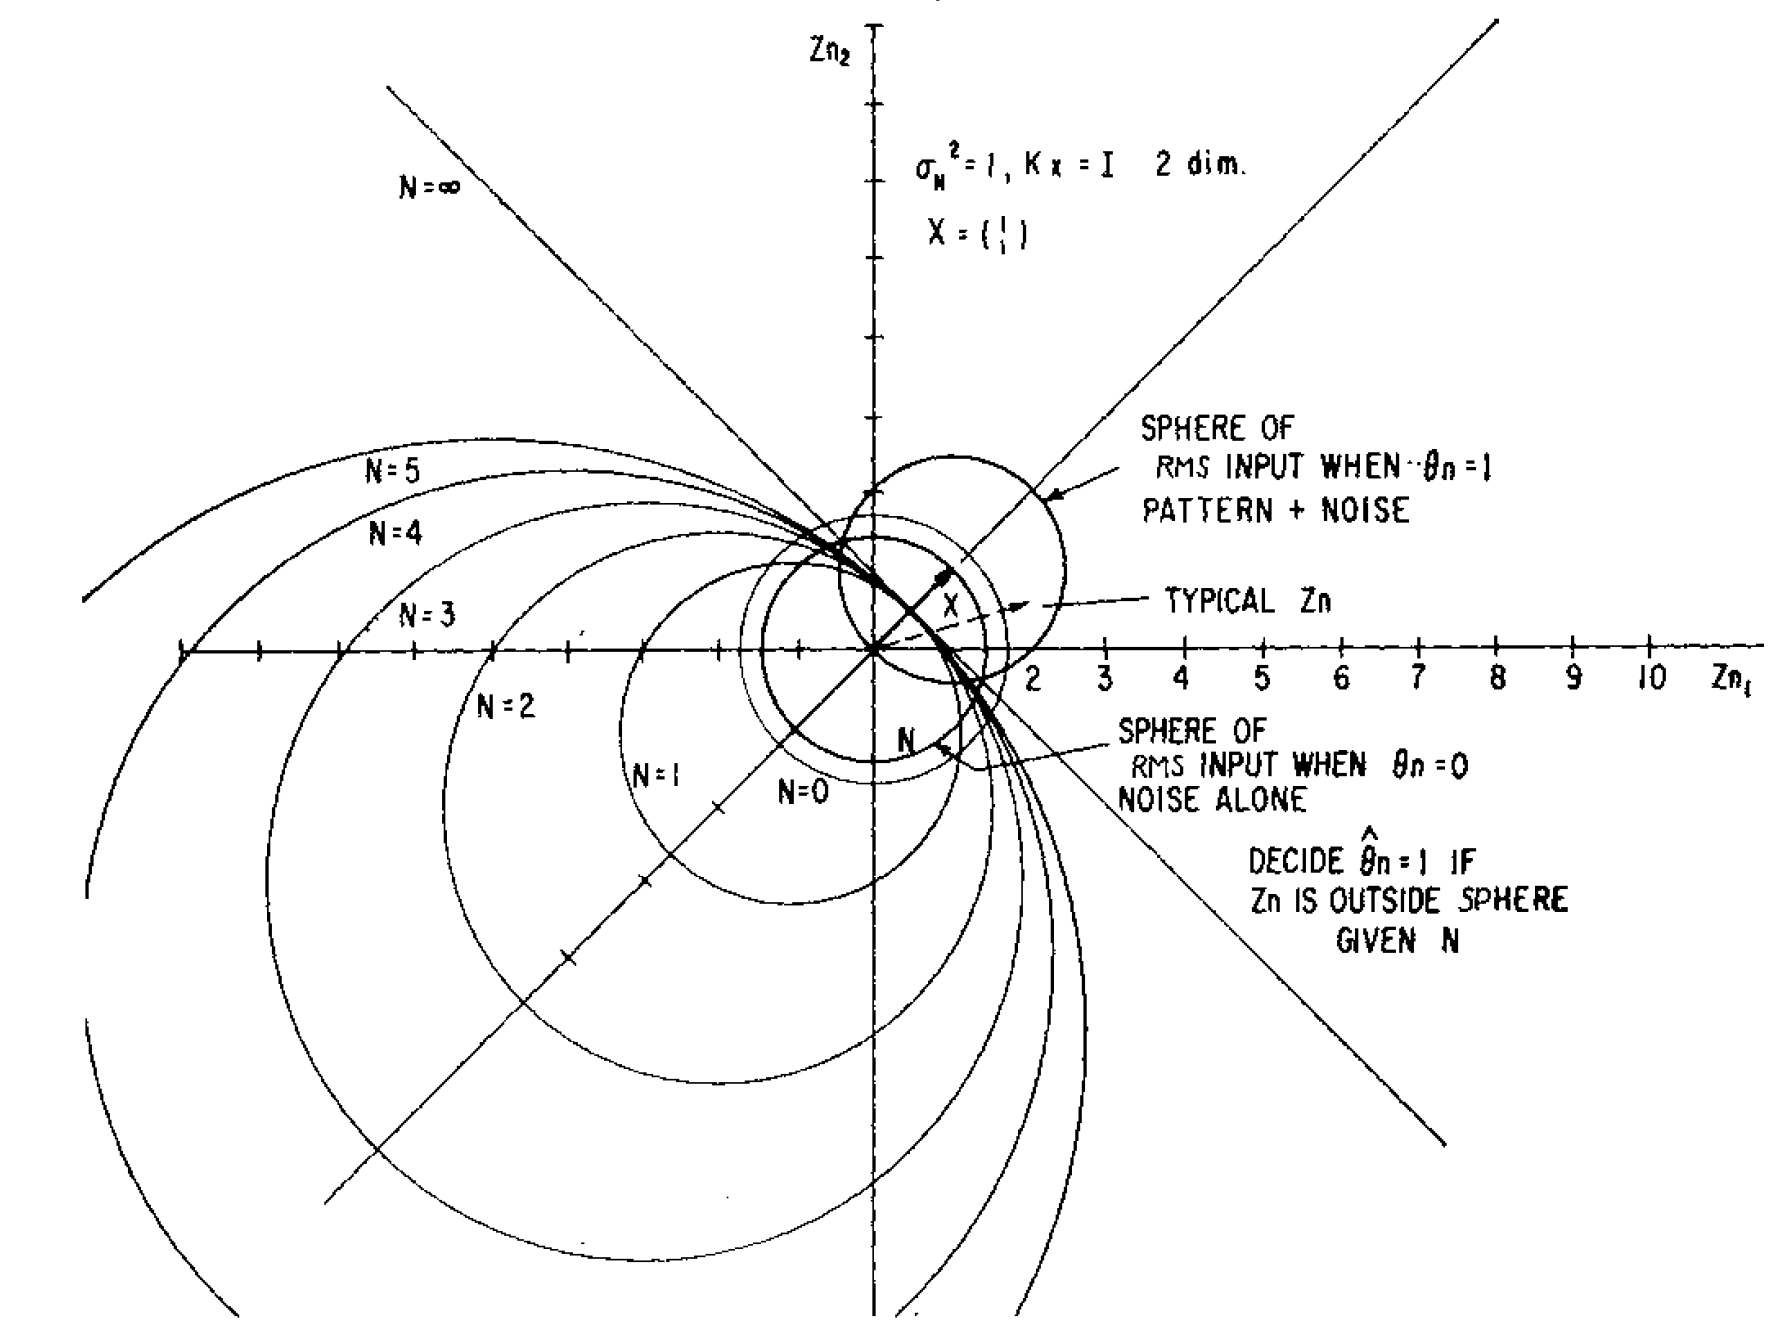
\includegraphics[width=\textwidth]{figs/scudder1965fig2.png}

        \begin{tiny}
          Fig. 2, ``Probability of Error of Some Adaptive
          Pattern-Recognition Machines'', (c) IEEE, 1965
        \end{tiny}
      \end{center}
    \end{column}
  \end{columns}
\end{frame}


\begin{frame}
  \frametitle{The Self-supervised Case}

  Now, consider the self-supervised case.  We don't know $X$, and we
  don't know $\theta_n$.  Instead, all we have is our own classifier
  output, $\hat\theta_n$, at each time step.  Can we learn the optimum classifier?
  \begin{itemize}
  \item Calculate the log likelihood ratio (LLR):
    \begin{displaymath}
      Q_n = Z_nK_n^{-1}Z_n -
      (Z_n-H_n)^T(K_N+K_n)^{-1}(Z_n-H_n)
    \end{displaymath}
  \item Threshold the log likelihood ratio:
    \begin{displaymath}
      \hat\theta_n = \left\{\begin{array}{ll}
      1 & Q_n > \text{threshold}\\
      0 & Q_n \le \text{threshold}
      \end{array}\right.
    \end{displaymath}
  \item Update the matched filter covariance estimate:
    \begin{displaymath}
      K_{n+1} = \left(K_n^{-1}+\hat\theta_n K_N^{-1}\right)^{-1}
    \end{displaymath}
  \item Update the matched filter estimate:
    \begin{displaymath}
      H_{n+1} = H_n + K_N^{-1}K_{n+1}(Z_n-H_n)\hat\theta_n
    \end{displaymath}
  \end{itemize}
\end{frame}

\begin{frame}
  \begin{columns}
    \begin{column}{0.4\textwidth}
      
      Figure at right shows the {\bf supervised} case.  Can we match it
      using a {\bf self-supervised} learner?
      \begin{itemize}
      \item The $n=0$ classifier is still a circle: any {\bf small}
        vector is classified as $\hat\theta_n=0$, any {\bf large}
        vector is classified as $\hat\theta_n=1$.
      \item This is a good thing!  Some of the large vectors are,
        indeed, signals.  But not all!
      \end{itemize}
    \end{column}
    \begin{column}{0.6\textwidth}
      \begin{center}
        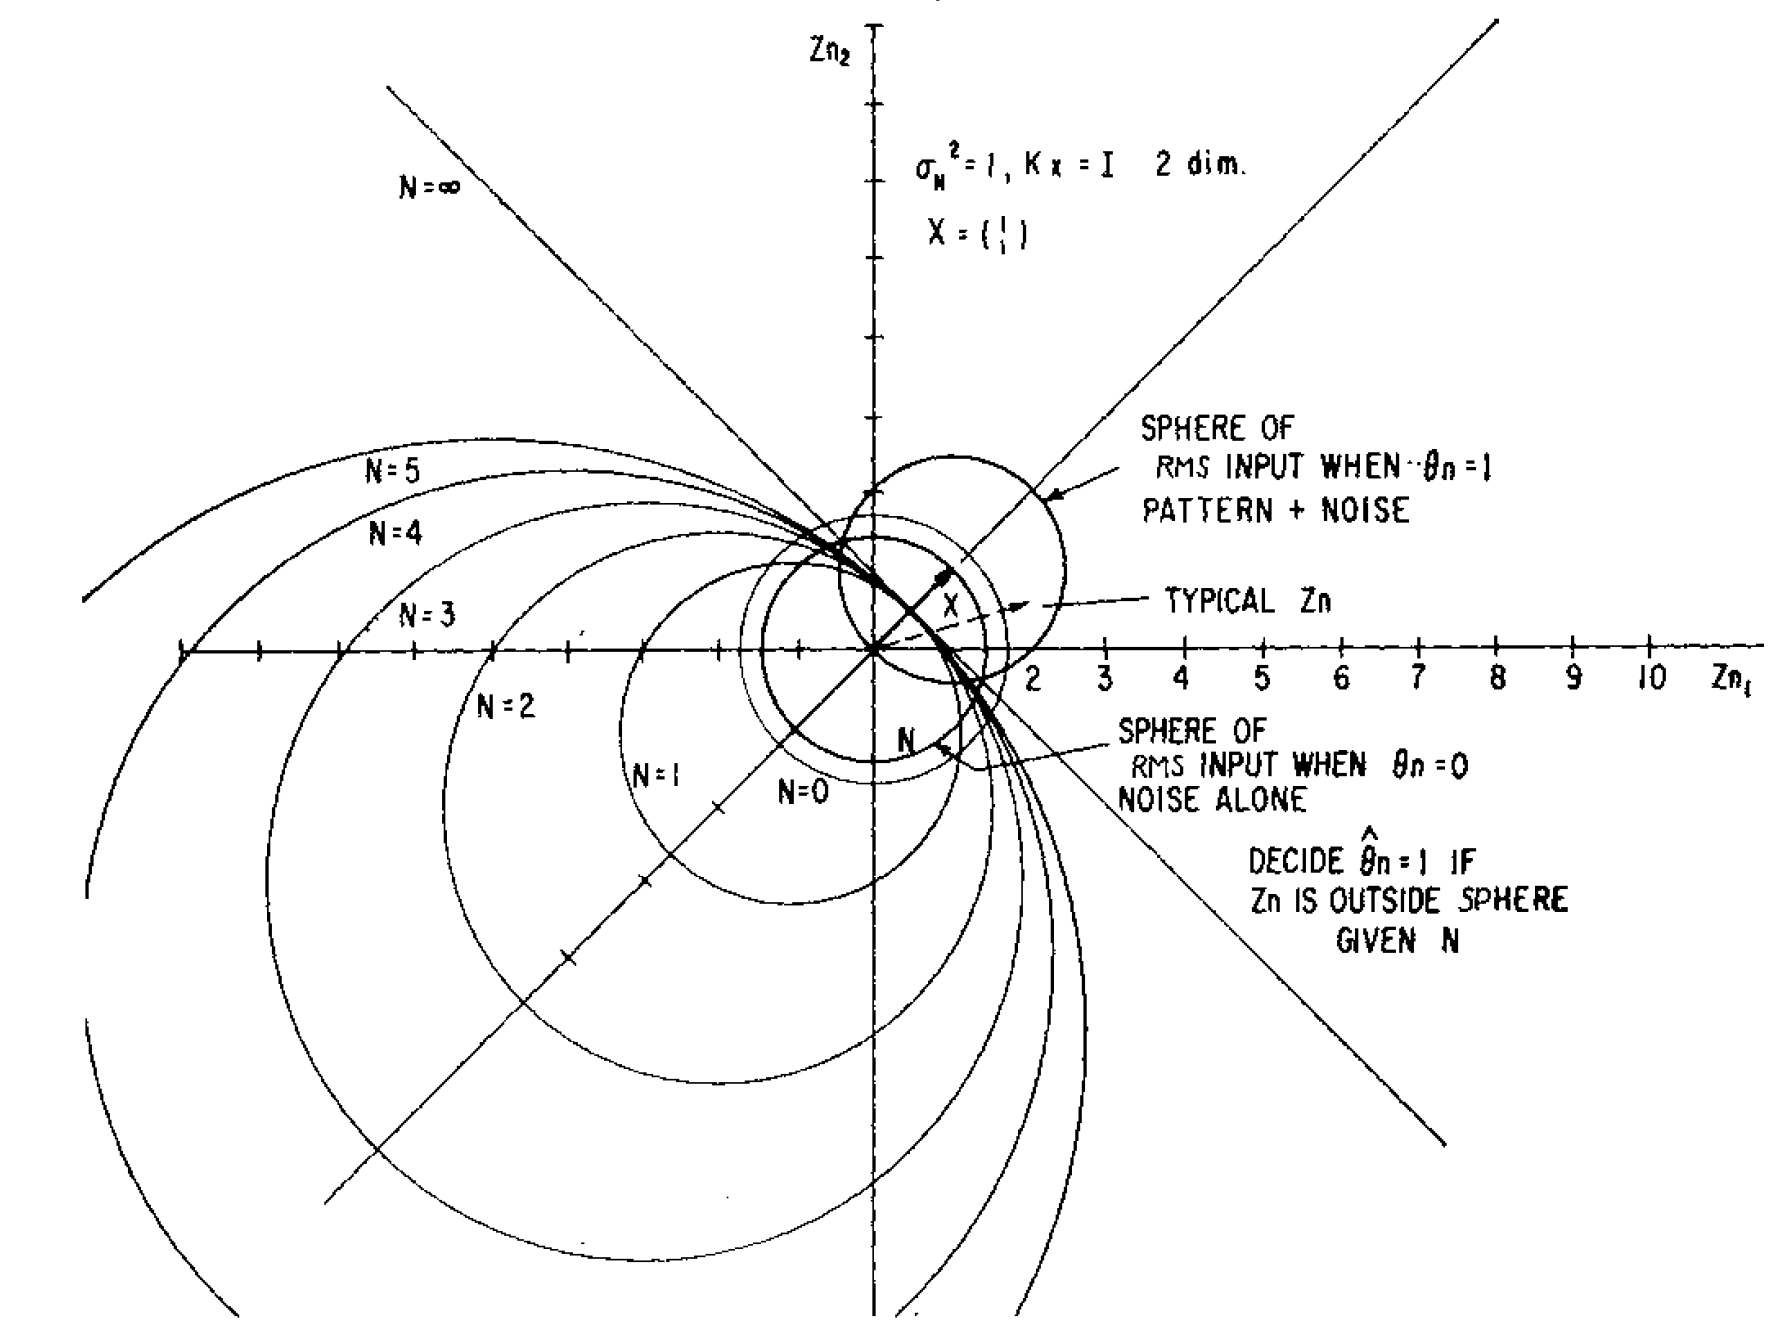
\includegraphics[width=\textwidth]{figs/scudder1965fig2.png}

        \begin{tiny}
          Fig. 2, ``Probability of Error of Some Adaptive
          Pattern-Recognition Machines'', (c) IEEE, 1965
        \end{tiny}
      \end{center}
    \end{column}
  \end{columns}
\end{frame}


\begin{frame}
  \begin{columns}
    \begin{column}{0.4\textwidth}

      The self-supervised learner learns a ``matched filter,'' $H_n$,
      such that
      \begin{itemize}
      \item The hyperplane is $H_n^TZ_n = \text{threshold}$.
      \item $H_n$ is the average of all of the $Z$ vectors on the
        right side of the hyperplane.
      \end{itemize}
    \end{column}
    \begin{column}{0.6\textwidth}
      \begin{center}
        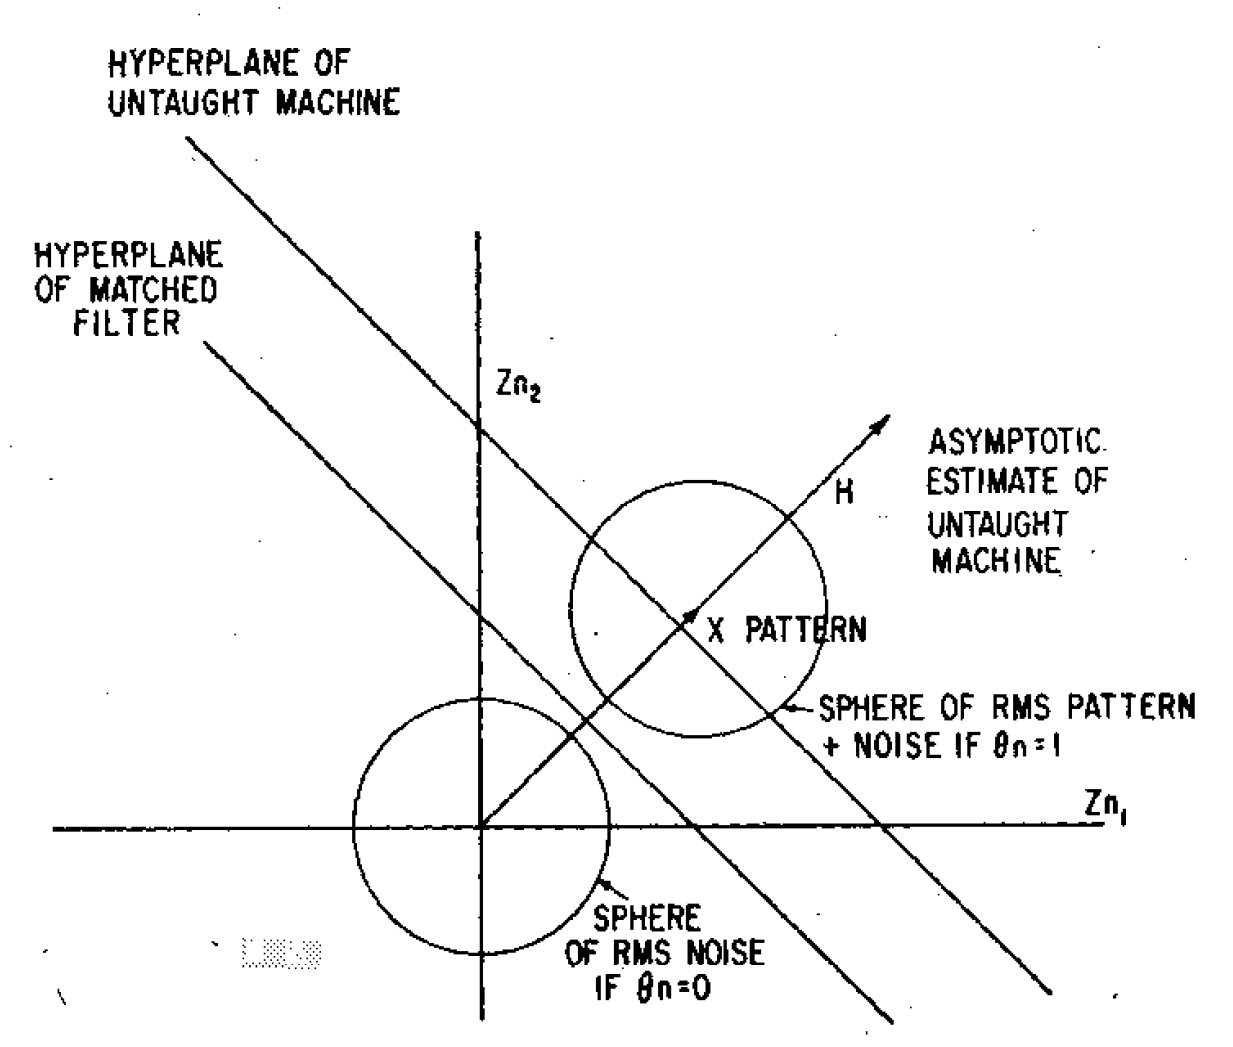
\includegraphics[width=\textwidth]{figs/scudder1965fig4.png}

        \begin{tiny}
          Fig. 4, ``Probability of Error of Some Adaptive
          Pattern-Recognition Machines'', (c) IEEE, 1965
        \end{tiny}
      \end{center}
    \end{column}
  \end{columns}
\end{frame}

\begin{frame}
  \frametitle{Summary: Scudder's Theory of Self-Supervised Learning}

  \begin{itemize}
  \item The classifier learns to call all big vectors ``signal,'' and
    all small vectors ``noise.''
  \item It is biased: small signal vectors get misclassified as ``noise.''
  \item There is a threshold effect: if the noise covariance matrix,
    $K_N$, is too large, then the learner fails to converge.
  \end{itemize}
\end{frame}

%%%%%%%%%%%%%%%%%%%%%%%%%%%%%%%%%%%%%%%%%%%%
\section[APC]{Autoregressive Language Modeling \& Autoregressive Predictive Coding}
\setcounter{subsection}{1}

\begin{frame}
  \frametitle{The N-Gram Language Model}

  Claude Shannon (``A Mathematical Theory of Communication,'' 1948)
  proposed representing the probability of a sentence,
  $w=[w_1,\ldots,w_L]$ as the product of its N-gram probabilities:
  \begin{displaymath}
    P(w) = \prod_{i=1}^L P(w_i|w_{i-1},\ldots,w_1)
    \approx\prod_{i=1}^L P(w_i|w_{i-1},\ldots,w_{i-N+1})
  \end{displaymath}
  He proposed storing these probabilities in a lookup table, and using
  them to verify a transmitted message.
\end{frame}

\begin{frame}
  \frametitle{The N-Gram Language Model}

  Shannon proposed that pseudo-sentences can be generated by sampling
  from these N-gram probability tables:
  \begin{itemize}
  \item Sentence generated by sampling from unigram (1-gram) probability tables:
    \begin{center}
      REPRESENTING AND SPEEDILY IS AN GOOD APT OR COME CAN DIFFERENT NATURAL
      HERE HE THE A IN CAME THE TO OF TO EXPERT GRAY COME TO FURNISHES
      THE LINE MESSAGE HAD BE THESE.
    \end{center}
  \item Sentence generated by sampling from unigram (2-gram) probability tables:
    \begin{center}
      THE HEAD AND IN FRONTAL ATTACK ON AN ENGLISH WRITER THAT THE CHARACTER
      OF THIS POINT IS THEREFORE ANOTHER METHOD FOR THE LETTERS THAT
      THE TIME OF WHO EVER TOLD THE PROBLEM FOR AN UNEXPECTED.
    \end{center}
  \end{itemize}
\end{frame}

\begin{frame}
  \frametitle{Autoregressive Neural Language Model}

  An autoregressive neural language model expresses each word as a
  learned vector.  The vector corresponding to word $w$ is
  $x(w)=[x_1(w),\ldots,x_d(w)]$, whose elements $x_i(w)$ are learned
  parameters.  The parameters $x(w)$, $\phi$ and $\theta$ are then
  learned in order to minimize the cross-entropy loss:
  \begin{displaymath}
    {\mathcal L}=-\sum_{i=1}^L \ln P(w_i|w_{i-1},\ldots,w_1)
  \end{displaymath}
  which is computed using an LSTM or Transformer as:
  \begin{align*}
    P(w_i|w_{i-1},\ldots,w_1) &= \frac{\exp\left(\text{Score}(w_i,h_i;\phi)\right)}{\sum_w \exp\left(\text{Score}(w,h_i;\phi)\right)} \\
    h_i &= f\left(x(w_{i-1}),\ldots,x(w_1);\theta\right)
  \end{align*}
\end{frame}

\begin{frame}
  \frametitle{Autoregressive Neural Language Model}

  Autoregressive language modeling performance varies dramatically
  depending on the number of parameters of the neural net.

  \begin{itemize}
  \item GPT-2 (1.5 billion params): sometimes ``In practice, he was a
    very conservative figure, but he was also a very conservative
    figure in the sense that he was a very conservative figure in the
    sense that he was a very conservative figure\ldots''
  \item GPT-3 (175 billion params): \url{https://maraoz.com/2020/07/18/openai-gpt3/}:
``So there are lots of posts for GPT-3 to study and learn
    from. The forum also has many people I don’t like. I expect them
    to be disproportionately excited by the possibility of having a
    new poster that appears to be intelligent and relevant. I’ve
    been following the forum for years. There are many posts I know
    the answers to, so I could provide a quick response and measure
    how well GPT-3 does with comments similar to those I make.''
  \end{itemize}
\end{frame}

\begin{frame}
  \frametitle{Autoregressive Predictive Coding (Chung and Glass, 2021)}

  \begin{itemize}
  \item In an autoregressive language model, the word representations,
    $x(w)$, and the LSTM or Transformer state vectors, $h_i$, are
    summaries of the context-independent and context-dependent meaning
    of a word, respectively.
  \item Chung and Glass (2020) proposed ``Autoregressive Predictive
    Coding'' to compute similar representations for speech.
  \end{itemize}
\end{frame}

\begin{frame}
  \frametitle{Autoregressive Predictive Coding (Chung and Glass, 2021)}

  APC trains a transformer so that its last layer, $h_L$, can be used
  to predict the input vector $n$ steps later:
  \begin{align*}
    h_0 &= W_{in}x + P(x)\\
    h_l &= \text{Transformer}(h_{l-1})\\
    y &= W_{out}h_L\\
    {\mathcal L} &= \sum_{i=1}^{N-n}\left|x_{i+n}-y_i\right|
  \end{align*}
  
\end{frame}

\begin{frame}
  \frametitle{How is it used?}

  \begin{itemize}
  \item The neural net is first {\bf pre-trained} using the
    autoregressive criterion on the previous page, using only the
    inputs (the audio).
  \item The system is then connected to a few extra layers of neural
    net, in order to perform some downstream task.  Either:
    \begin{itemize}
    \item The pre-trained network may be {\bf frozen}, in which case
      only the extra layers are trained using downstream labels, or
    \item The pre-trained network is {\bf fine-tuned} (trained in
      order to optimize performance on the downstream task.
    \end{itemize}
  \item These ideas (frozen vs. fine-tuned) were laid out in BERT, so
    let's look at BERT.
  \end{itemize}
\end{frame}


%%%%%%%%%%%%%%%%%%%%%%%%%%%%%%%%%%%%%%%%%%%%
\section[BERT]{BERT: Masked Language Modeling \& Masked Predictive Coding}
\setcounter{subsection}{1}

\begin{frame}
  \frametitle{The BERT ecosystem: Pre-training and Fine-tuning}

  BERT stands for Bidirectional Encoder Representations from
  Transformers.  The idea is to pre-train an encoder, which can then
  be fine-tuned for downstream tasks:
  \centerline{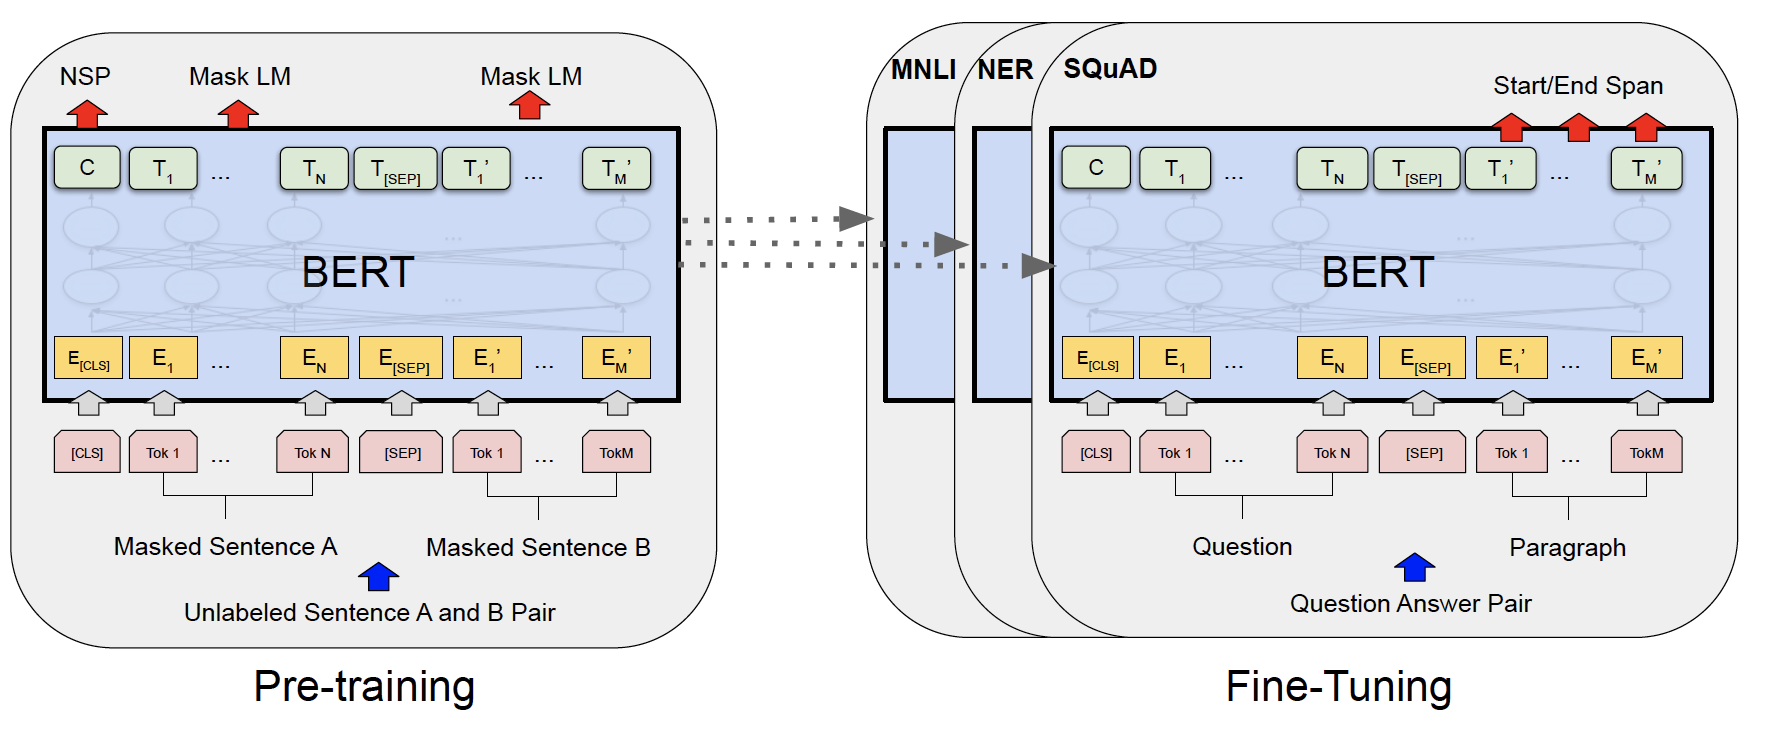
\includegraphics[width=\textwidth]{figs/devlin2018fig1.png}}
  \centerline{\tiny Devlin et al., 2018}
\end{frame}

\begin{frame}
  \frametitle{Pre-Training: Masked Language Modeling}

  The pre-training criterion is masked language modeling.
  \begin{displaymath}
    m_i = \left\{\begin{array}{ll}
    1 & \text{word}~i~\text{is visible (probability: 85\%)}\\
    0 & \text{word}~i~\text{is masked (probability: 15\%)}
    \end{array}\right.
  \end{displaymath}
  Then, from input vectors $e_1,\ldots, e_n$ and masked-word
  replacement noises $v_1,\ldots, v_n$, the transformer computes
  outputs
  \begin{displaymath}
    t_i = \text{Transformer}\left(m_1e_1+(1-m_1)v_1,\ldots,m_ne_n+(1-m_n)v_n\right)
  \end{displaymath}
  The loss function measures the ability of the model to predict the
  masked words only.
  \begin{displaymath}
    {\mathcal L}=-\sum_{i=1}^n (1-m_i)\ln
    \left(\frac{\exp\left(\text{Score}(At_i,e_i)\right)}{\sum_E\exp\left(\text{Score}(At_i,e)\right)}
    \right),
  \end{displaymath}
  where $A$ is the matrix of softmax weights.
\end{frame}

\begin{frame}
  \frametitle{Hidden Unit BERT (HuBERT)}

  HuBERT uses the masked language modeling idea, but instead of words,
  it predict units such as K-means clusters of mel frequency cepstral
  coefficients (MFCC).
  \centerline{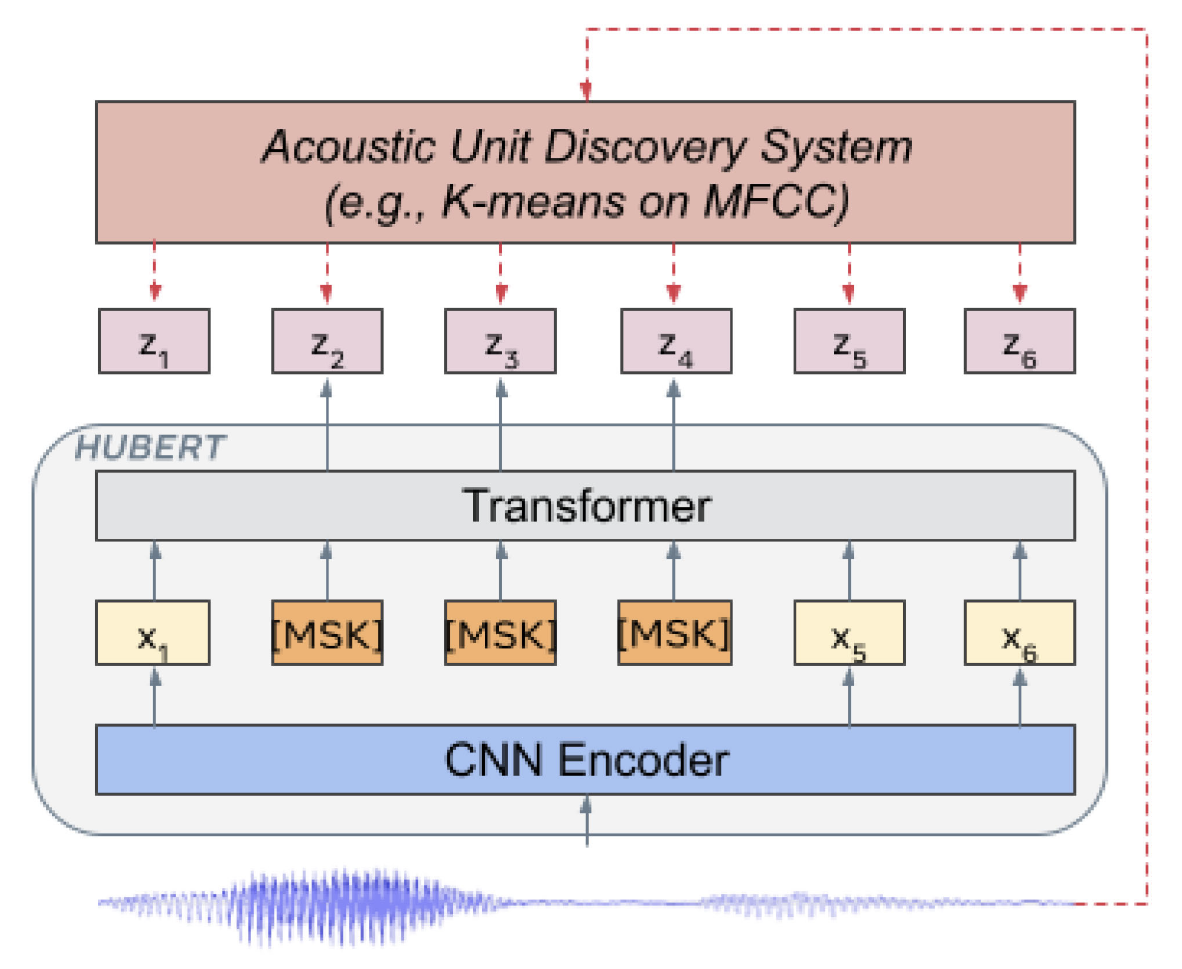
\includegraphics[width=0.6\textwidth]{figs/hsu2021fig1.png}}
  \centerline{\tiny Hsu et al., 2021, Fig. 1}
\end{frame}

\begin{frame}
  \frametitle{HuBERT notation}

  \begin{itemize}
  \item $X=[x_1,\ldots,x_T]$ are the frames of a speech utterance,
    $x_t\in\Re^d$,
  \item $h(X)=Z=[z_1,\ldots,z_T]$ are the hidden units computed from
    $X$, $z_t\in\{1,\ldots,C\}$ where $C$ is the number of categories.
  \item $M\subset\{1,\ldots,T\}$ are the frames to be masked.
  \item $\tilde{X}$ is the masked sequence, i.e., masked frames are
    replaced by a ``MASK'' token.
  \end{itemize}
\end{frame}

\begin{frame}
  \frametitle{HuBERT: Masked language modeling loss function}

  The loss function is
  \begin{displaymath}
    L(f;X,M,Z) = -\sum_{t\in M} \ln p(z_t|\tilde{X},t),
  \end{displaymath}
  where the probability is computed using a softmax:
  \begin{displaymath}
    p(c|\tilde{X},t) = \frac{\exp\left(\text{Score}(Ao_t,e_c)\right)}{\sum_{c'=1}^C\exp\left(\text{Score}(Ao_t,e_{c'})\right)},
  \end{displaymath}
  where $A$ is the softmax weight matrix, $o_t$ is the transformer
  output, and $e_c$ is an embedding learned for hidden unit $c$.
\end{frame}

\begin{frame}
  \frametitle{HuBERT: Fine tuning}

  \begin{itemize}
  \item The transformer is trained so that its outputs, $o_t$, best
    predict the hidden units, $z_t$.
  \item The hidden units are then discarded; the softmax weights $A$
    and the transformer $o_t$ are trained to minimize
    \begin{displaymath}
      L_{\text{CTC}}(Y|X) + w_1 L_{\text{LM}}(Y) + w_2|Y|
    \end{displaymath}
  \end{itemize}
\end{frame}

\begin{frame}
  \frametitle{Why it works}

  \begin{itemize}
  \item The transformer is trained so that it accumulates information
    from context ($o_t$) in order to optimally predict a quantized unit.
  \item The quantized units are kind of like phonemes, so a
    Transformer that predicts them well is also good at predicting
    phonemes.
  \item 
    The more phoneme-like the hidden units are, the more effective the
    pre-training works.  The best procedure is:
    \begin{enumerate}
    \item K-means cluster the MFCC; pre-train HuBERT to predict that.
    \item K-means cluster the first-round HuBERT vectors; pre-train another HuBERT.
    \item K-means cluster the second-round HuBERT vectors; pre-train another HuBERT.
    \item Fine tune as an ASR.
    \end{enumerate}
  \end{itemize}
\end{frame}

%%%%%%%%%%%%%%%%%%%%%%%%%%%%%%%%%%%%%%%%%%%%
\section[CPC]{Contrastive Predictive Coding \& Wav2vec}
\setcounter{subsection}{1}

\begin{frame}
  \frametitle{Contrastive Predictive Coding (CPC)}

  Contrastive predictive coding was originally a form of autoregressive prediction:

  \centerline{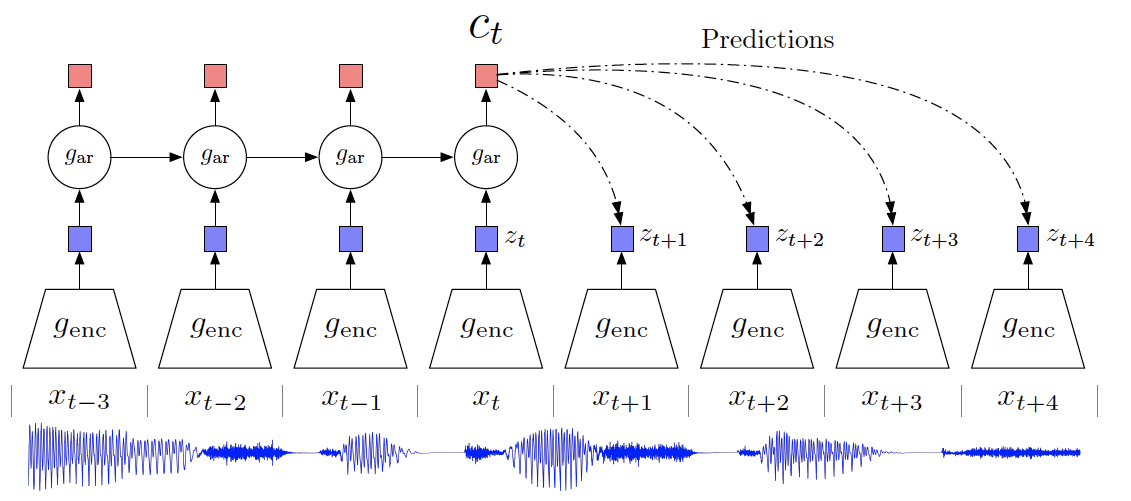
\includegraphics[width=\textwidth]{figs/oord2018fig1.png}}

  \centerline{\tiny Oord et al., 2018, Fig. 1}
\end{frame}

\begin{frame}
  \frametitle{The ``Contrastive'' in CPC}

  The key innovation in CPC is the loss term.  A normal autoregressive
  language model trains $c_t$ in order to minimize
  \begin{displaymath}
    {\mathcal L}_{\text{ALM}} = -\sum_t \ln\frac{\exp\left(\text{Score}(x_{t+k},c_t)\right)}{\sum_{x\in V}\exp\left(\text{Score}(x,c_t)\right)},
  \end{displaymath}
  where $V$ is the entire vocabulary (all possible words).  By
  contrast, CPC trains $c_t$ in order to minimize
  \begin{displaymath}
    {\mathcal L}_{\text{CPC}} = -\sum_t \ln\frac{\exp\left(\text{Score}(x_{t+k},c_t)\right)}{\sum_{x\in X}\exp\left(\text{Score}(x,c_t)\right)}
  \end{displaymath}
  where $X=\{x_1,\ldots,x_N\}$ is a set of $N$ randomly chosen
  negative examples.
\end{frame}

\begin{frame}
  \frametitle{CPC can predict either continuous or discrete targets}

  \begin{itemize}
  \item 
    The language modeling criteria (autoregressive and MLM) require a
    discrete set of words.  CPC, by contrast, can predict continuous
    vectors.  The set of negative examples, $X=\{x_1,\ldots,x_N\}$,
    can be either continuous-valued or discrete; the only difference
    is the way $\text{Score}(x_{t+k},c_t)$ is computed.
  \item
    The original CPC paper (Oord, 2018) used continuous vectors for
    speech and images, and discrete words for NLP applications.
  \item
    Wav2vec 2.0 tested both continuous and discrete speech targets,
    and found that discrete targets worked better, possibly because
    they force the transformer to learn to predict something
    phoneme-like.
  \end{itemize}
\end{frame}

\begin{frame}
  \frametitle{wav2vec 2.0 (Baevski et al., 2020)}

  \centerline{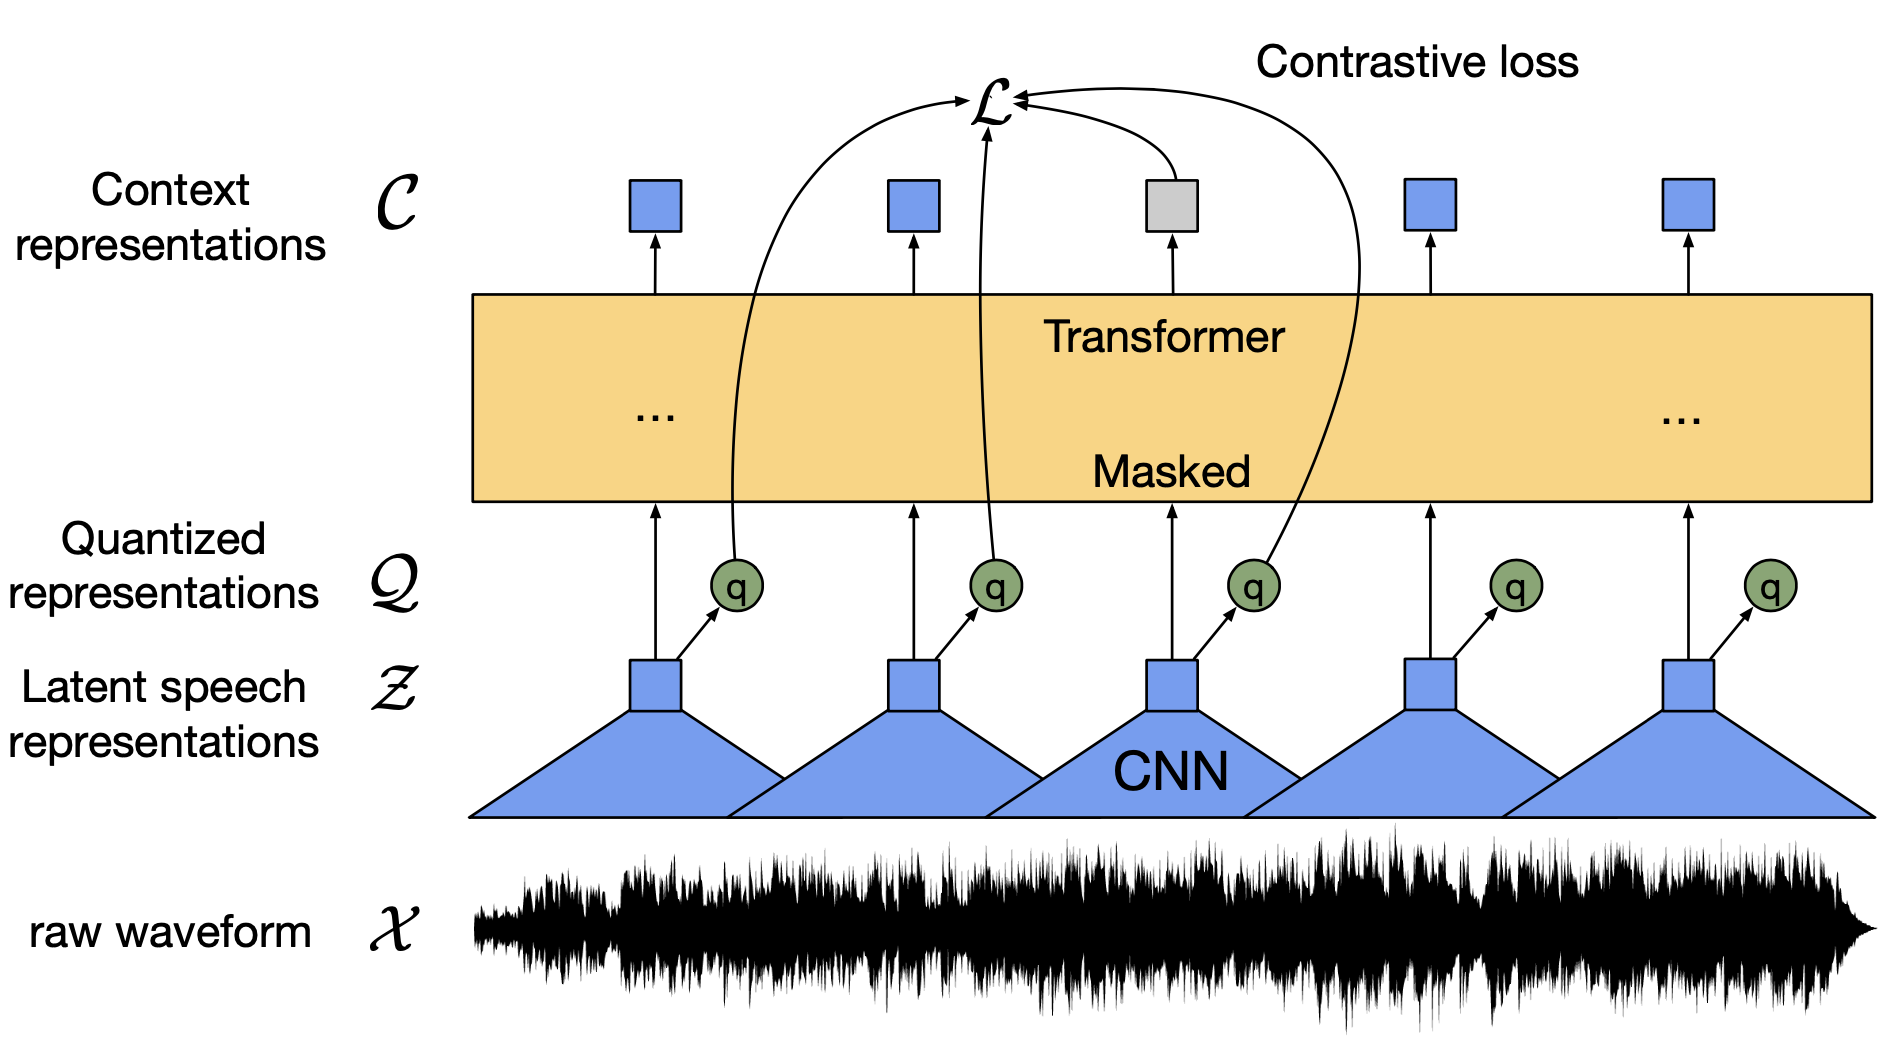
\includegraphics[width=\textwidth]{figs/baevski2020fig1.png}}

  \centerline{\tiny Baevski et al., 2020}
\end{frame}

\begin{frame}
  \frametitle{wav2vec 2.0: Loss Function}

  \begin{displaymath}
    {\mathcal L}=-\ln\frac{\exp\left(\text{Score}(c_t,q_t)\right)}{\sum_{q\in Q_t}\exp\left(\text{Score}(c_t,q_t)\right)},
  \end{displaymath}
  where $q_t$ is quantized (codebook index), but $Q_t$ is a set of negative examples.
\end{frame}

\begin{frame}
  \frametitle{wav2vec 2.0: Other Details}

  Unlike HuBERT, the quantizer functions $q_t=Q(z_t)$ is learned along
  with the other parameters (instead of being a K-means learned
  offline).  It's therefore necessary to prevent the trivial failure
  mode in which all inputs are mapped to the same codevector.  To
  prevent this, wav2vec 2.0 adds a {\bf diversity loss}, equal to the negative
  entropy of the codevector indices $q_1,\ldots,q_T$.  If they are all
  the same, the entropy is zero; if they are all different, the
  entropy is maximized (and loss is minimized):
  \begin{align*}
    {\mathcal L}_d &= -\frac{1}{V}H(p) = \frac{1}{V}\sum_{v=1}^V p_v\log p_v\\
    p_v &= \frac{1}{T}\sum_{t=1}^T \left(1~\text{iff}~q_t=v\right)
  \end{align*}
  
\end{frame}


%%%%%%%%%%%%%%%%%%%%%%%%%%%%%%%%%%%%%%%%%%%%
\section[Summary]{Summary}
\setcounter{subsection}{1}



\begin{frame}
  \frametitle{A Brief History of Self-Supervised Learning for NLP}

  \begin{itemize}
  \item {\bf Autoregressive Neural Language Modeling:} Many papers,
    e.g., ``LSTM neural networks for language modeling,'' Sundermeyer,
    Schl{\"{u}}ter \& Ney, 2012
    \begin{displaymath}
      {\mathcal L}=-\sum_{i=1}^L \ln P(w_i|w_{i-1},\ldots,w_1)
    \end{displaymath}
  \item {\bf Masked Language Modeling (BERT):} ``BERT: Pre-training of
    Deep Bidirectional Transformers for Language Understanding,''
    Devlin, Chang, Lee \& Toutanova, 2018
    \begin{displaymath}
      {\mathcal L}=-\sum_{i=1}^n (1-m_i)\ln
      \left(\frac{\exp\left(\text{Score}(At_i,e_i)\right)}{\sum_E\exp\left(\text{Score}(At_i,e)\right)}
      \right),
    \end{displaymath}
  \item {\bf Contrastive Predictive Coding:} ``Representation Learning with
    Contrastive Predictive Coding,'' Oord, Li \& Vinyals, 2018
    \begin{displaymath}
      {\mathcal L}_{\text{CPC}} = -\sum_t \ln\frac{\exp\left(\text{Score}(x_{t+k},c_t)\right)}{\sum_{x\in X}\exp\left(\text{Score}(x,c_t)\right)}
    \end{displaymath}
  \end{itemize}
\end{frame}


\begin{frame}
  \frametitle{A Brief History of Self-Supervised Learning for Speech}

  \begin{itemize}
  \item {\bf Contrastive Predictive Coding:} ``Representation Learning with
    Contrastive Predictive Coding,'' Oord, Li \& Vinyals, 2018
    \begin{displaymath}
      {\mathcal L}_{\text{CPC}} = -\sum_t \ln\frac{\exp\left(\text{Score}(x_{t+k},c_t)\right)}{\sum_{x\in X}\exp\left(\text{Score}(x,c_t)\right)}
    \end{displaymath}
  \item {\bf Autoregressive Predictive Coding:} ``Generative
    Pre-training for Speech with Autoregressive Predictive Coding,''
    Chung \& Glass, 2020
    \begin{displaymath}
      {\mathcal L} = \sum_{i=1}^{N-n}\left|x_{i+n}-y_i\right|
    \end{displaymath}
  \item {\bf Masked Language Modeling (HuBERT):} ``HuBERT:
    Self-Supervised Speech Representation Learning by Masked
    Prediction of Hidden Units,'' Hsu et al., 2021
    \begin{displaymath}
      {\mathcal L} = -\sum_{t\in M} \ln\frac{\exp\left(\text{Score}(Ao_t,e_c)\right)}{\sum_{c'=1}^C\exp\left(\text{Score}(Ao_t,e_{c'})\right)}
    \end{displaymath}
  \end{itemize}
\end{frame}


\end{document}

